\chapter{Hardware}

\section{Requerimientos}
Los requerimientos que deben cumplirse son los mismos que fueron definidos para el dispositivo AFE.
Es necesario poder leer y escribir tarjetas RFID, comunicarse con servidores STM, leer tarjetas de contacto (módulo de seguridad), informar al usuario de lo que ocurre a través de una interfaz simple.

\section{Arquitecturas estudiadas}
Se definieron varias alternativas como posible solución, y se fueron descartando a medida que se encontraron limitantes o que no se cumplieran los requerimientos exigidos.

A continuación se describen algunas de las posibles arquitecturas:

\begin{itemize}
\item[1 -] SBC + OpenPCD + microcontrolador + lector de tarjetas de contacto + display + buzzer + leds
Tanto el OpenPCD como el microcontrolador se conectan directamente por USB al SBC. El microcontrolador maneja el resto de los dispositivos (lector de tarjetas de contacto, display, buzzer y leds).

\begin{figure}[H]
\centering
  \begin{center}
  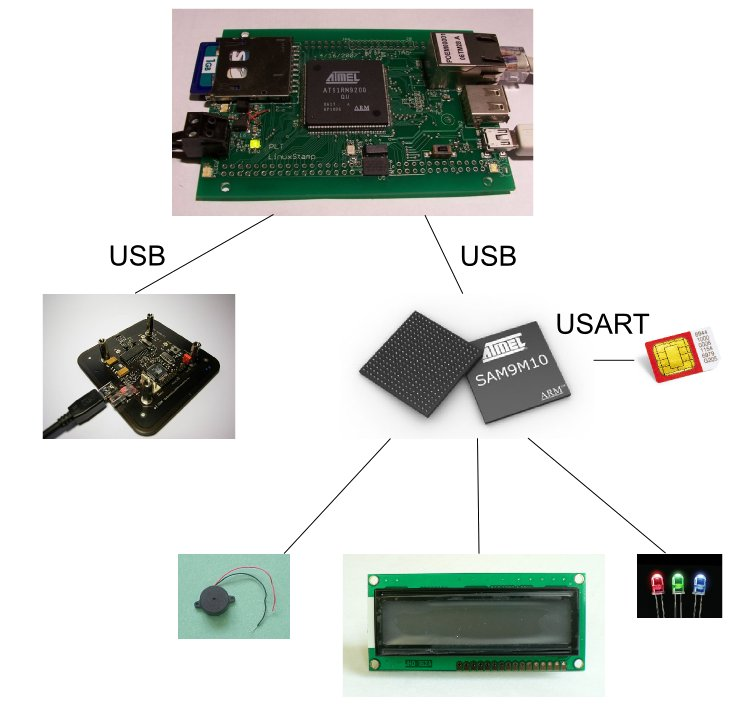
\includegraphics[scale=.25]{Imagenes/1.jpg} 
  \end{center}
  \caption{Solución posible 1}\label{Fig:HW} 
\end{figure}

Esta arquitectura tiene como ventaja el uso de la SBC que permite instalar un sistema operativo, reutilizar código ya implementado, posee varios puertos de E/S (I2C, USART, SPI, USB, GPIO, etc.), tiene gran capacidad de procesamiento, maneja memoria externa y brinda facilidad para realizar prototipos. Otra ventaja es el uso del microcontrolador que actúa como co-procesador, manejando el resto de los periféricos.

\item[2 -] SBC + OpenPCD + lector de tarjetas de contacto + display + buzzer + leds
El OpenPCD se conecta por USB a la SBC. La SBC maneja el resto de los dispositivos (lector de tarjetas de contacto, display, buzzer y leds) a través de sus interfaces nativas.

\begin{figure}[H]
\centering
  \begin{center}
  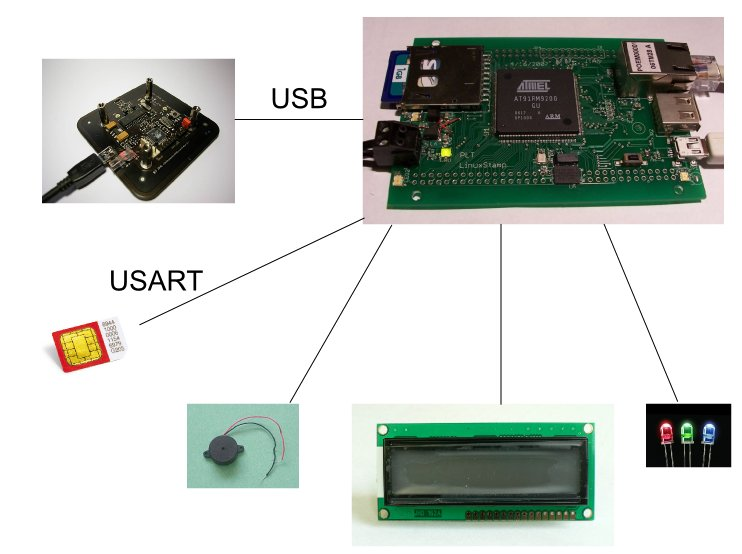
\includegraphics[scale=.25]{Imagenes/2.jpg} 
  \end{center}
  \caption{Solución posible 2}\label{Fig:HW} 
\end{figure}

\newpage

\item[3 -] SBC + lectores de tarjetas + display + buzzer + leds
Todos los periféricos (lectores de tarjetas, display, buzzer y leds) se conectan a la SBC a través de sus interfaces nativas, también el integrado CL RC632 de Philips que maneja la comunicación con las tarjetas sin contacto. Se diseña la antena para propagar RF.

\begin{figure}[H]
\centering
  \begin{center}
  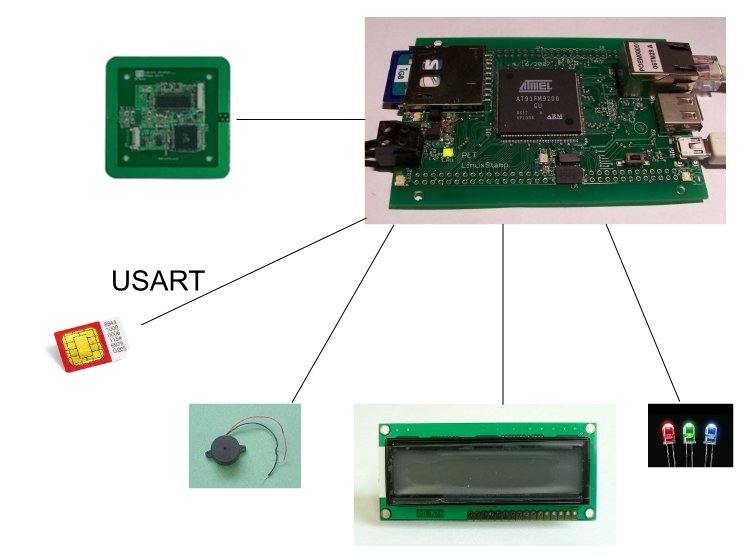
\includegraphics[scale=.25]{Imagenes/3.jpg} 
  \end{center}
  \caption{Solución posible 3}\label{Fig:HW} 
\end{figure}

\item[4 -] microcontrolador + lectores de tarjetas + display + buzzer + leds
Consta de un único PCB, que posee un microcontrolador como sistema central al cual se
conectan el resto de los dispositivos. Dicho PCB tiene incorporada la antena para la
propagación de RF. Se prevee el agregado de un modem 3G.

\begin{figure}[H]
\centering
  \begin{center}
  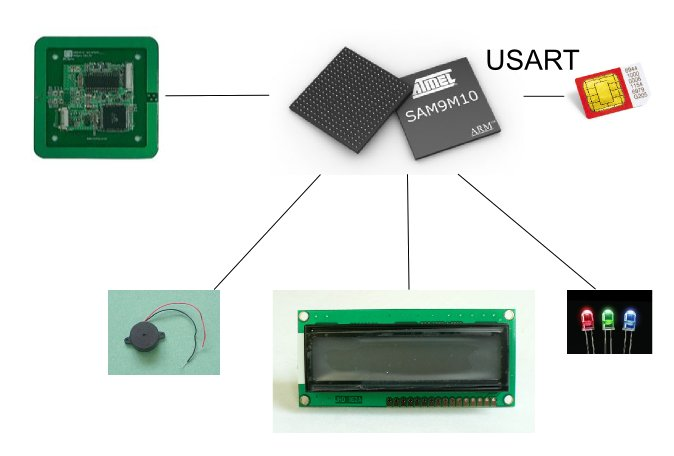
\includegraphics[scale=.25]{Imagenes/4.jpg} 
  \end{center}
  \caption{Solución posible 4}\label{Fig:HW} 
\end{figure}

\end{itemize}

\newpage
\section{Arquitectura seleccionada}
Luego de estudiar ventajas y desventajas de las arquitecturas planteadas, y discutirlo con los tutores, se eligieron dos de las posibilidades:

\begin{itemize}
\item SBC + OpenPCD + lector de tarjetas de contacto + display + buzzer + leds
\item SBC + lectores de tarjetas + display + buzzer + leds
\end{itemize}


\section{Elecci\'on de hardware, m\'odulos}
\subsection{SBC}
\subsection{VLT}
\subsection{Interfaz de Usuario}
\subsection{Lector de tarjetas de contacto}
\subsection{Lector-Escritor RFID}

\section{Funcionamiento general del prototipo}

\section{Funcionamiento de m\'odulos}
\subsection{SBC}
\subsection{VLT}
\subsection{Interfaz de Usuario}
\subsection{Lector de tarjetas de contacto}
\subsection{Lector-Escritor RFID}